%\subsubsection{Hubo2 Plus}
The Hubo2 Plus series robot is a 130 $cm$ (4' 3'') tall, 42 $kg$ (93 $lb$) full-size humanoid commonly refereed to as Hubo.  
The Hubo series was designed and constructed by Prof Jun-Ho Oh at the Hubo Lab in the Korean Advanced Institute of Science and Technology (KAIST) in Daejeon, South Korea \cite{1573587}.
Hubo has 2 arms, 2 legs and a head making it anthropomorphic to a human.
It contains 6 degrees of freedom (DOF) in each leg, 6 in each arm, 5 in each hand, 3 in the neck, and 1 in the waist; all totaling 38 DOF.
All joints of the major joints are high gain PID position controlled with the exception of the fingers.
The fingers are open-loop PWM controlled.
The sensing capability consists of a three axis force-torque (FT) sensor on each leg between the end of the ankle and the foot as well as between the arm where it connects to the hand.
Additionally it has an inertial measurement unit (IMU) at the center of mass and accelerometers on each foot.
The reference commands for all of the joints are sent from the primary control computer (x86) to the individual motor controllers via two Controller Area Network (CAN) buses.
This is the same communications bus found in most modern motor vehicles.
There are currently eight Hubo's functioning in the United States as of December 2012.
Four reside at Drexel University and one at Georgia Tech, Purdue, Ohio State and MIT.
Jaemi Hubo is the oldest of the Hubos in America and has been at the Drexel Autonomous Systems Lab\footnote{Drexel Autonomous Systems Lab: http://dasl.mem.drexel.edu/} (DASL) since 2008 \cite{jaemiHuboSRM}.
The name Jaemi Hubo comes from the phrase \textit{jaemi-gyopo} which means American born Korean.
Thus Jaemi Hubo means American Born Hubo or American Hubo.  
In addition Jaemi is an androgonous name in english and thus can be taken as either male or female. 
This is our social experiment see who call Jaemi, he, she or it.
Fig.~\ref{fig:hubo} shows the major dimensions of Hubo.
%(휴보) 

A full-scale safe testing environment designed for experiments with Jaemi Hubo was created using DASL's Systems Integrated Sensor Test Rig (SISTR)~\cite{5686325}.  
Additionally all algorithms are able to be tested on miniature and virtual versions of Jaemi Hubo prior to testing on the full-size humanoid through the creation of a surrogate testing platform for humanoids~\cite{5379582}.

\begin{figure}[thpb]
  \centering
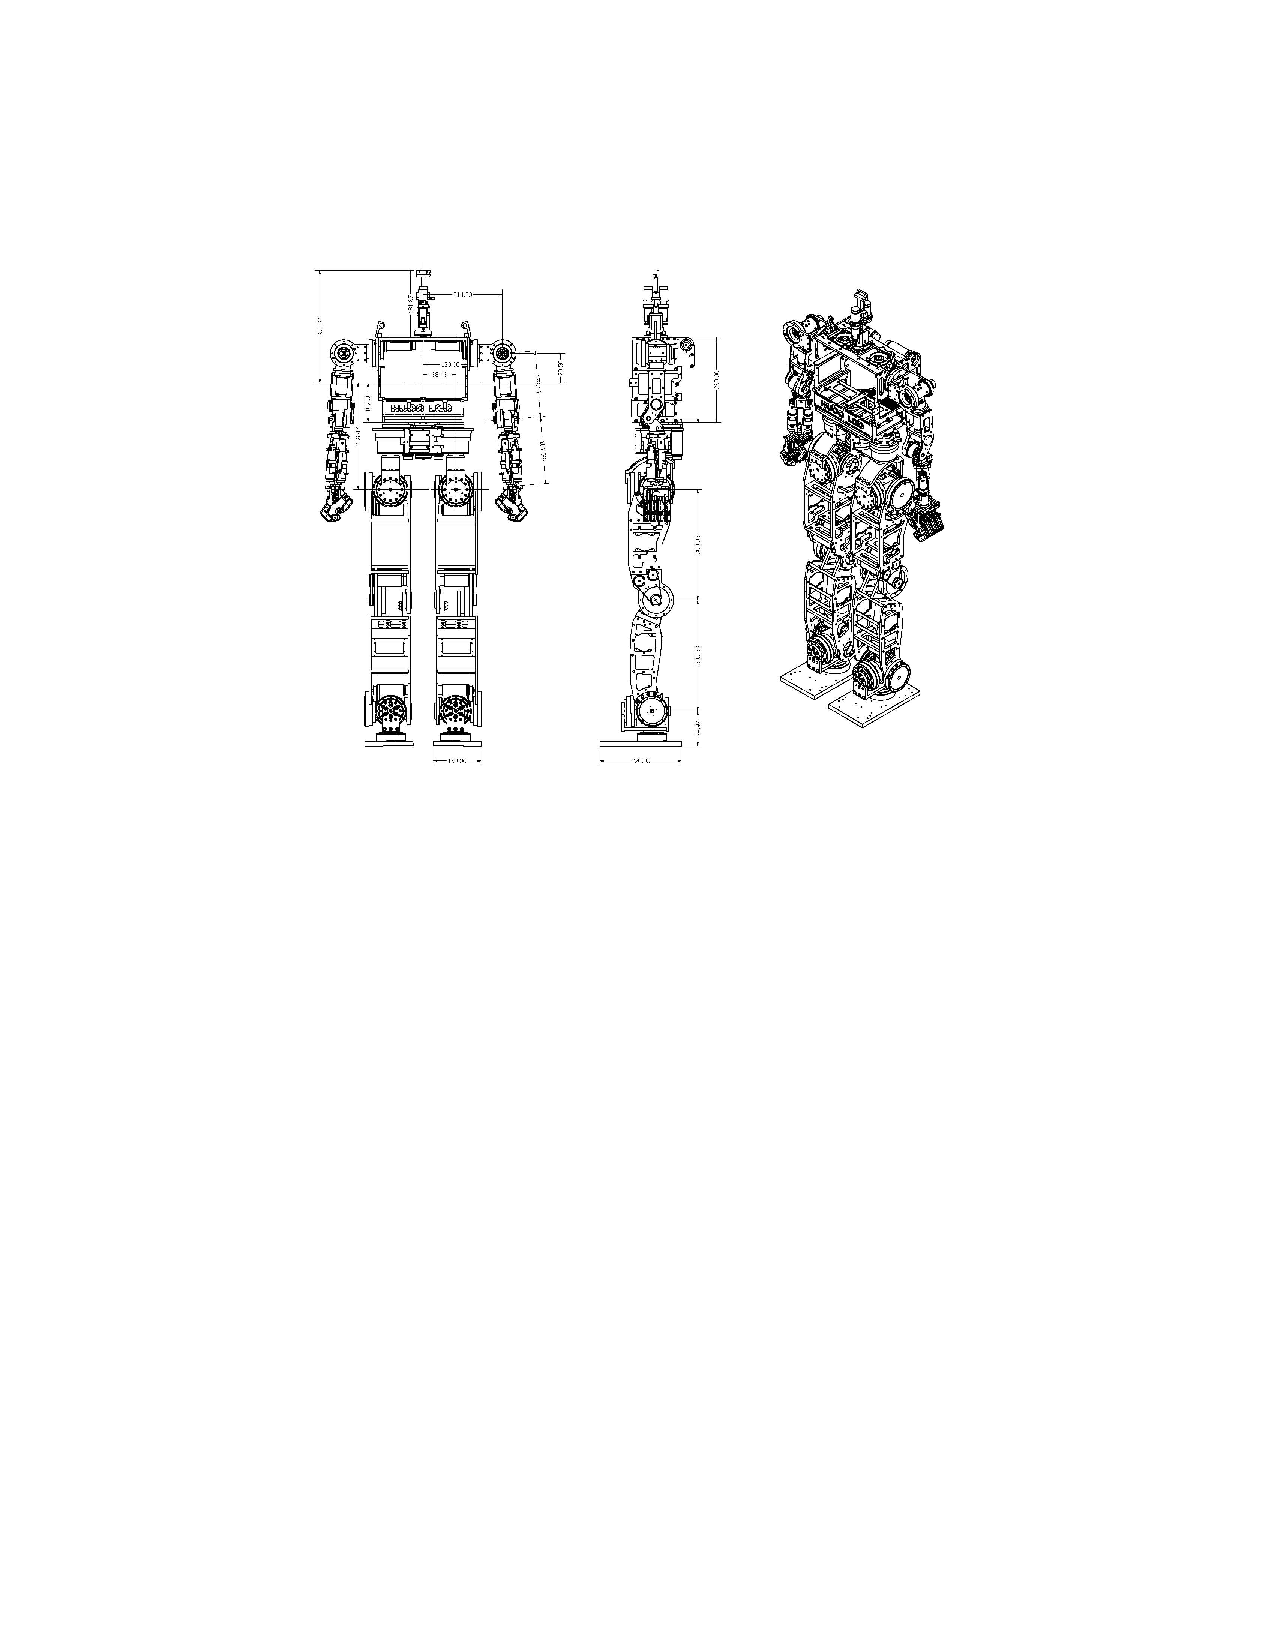
\includegraphics[width=1.0\columnwidth]{./pix/huboSkel.pdf}
  \caption{Hubo2 Plus platform: 38 DOF, 130 $cm$ tall full-size humanoid robot weighing 37 $kg$.}
  \label{fig:hubo}
\end{figure}



